\chapter{Implementation}
\label{ch:implementation}

We implemented our prototype in the LLVM framework, wasi-libc, and the wasmtime WebAssembly runtime.
The following sections detail the specific modifications and extensions we made to each component and some implementation choices and details to tackle specific problems.

\section{LLVM}
\label{sec:llvm}

We chose LLVM as our compiler from C/C++ to WebAssembly.
To be able to compile to our memory safety extension, we modified the WebAssembly backend to add support for our new instructions, allowing LLVM to emit our extension in both bytecode and text format.

\subsection{LLVM IR}
\label{subsec:llvm-ir}

In the middle end, we introduced three new intrinsic functions that correspond and are lowered to our \ac{WASM} instructions by the backend.
\begin{itemize}
  \item \lstinline[style=customc,language=llvm]{ptr @llvm.wasm.segment.new(ptr, i64)}
  \item \lstinline[style=customc,language=llvm]{void @llvm.wasm.segment.set_tag(ptr, ptr, i64)}
  \item \lstinline[style=customc,language=llvm]{void @llvm.wasm.segment.free(ptr, i64)}
\end{itemize}
The clang frontend or a sanitizer pass can insert calls to these intrinsic functions.
The following listing shows how we lower a function that allocates 32 bytes on the stack to LLVM IR.

\begin{lstlisting}[frame=h,style=customc,
  label={lst:llvm-intrinsics},language=llvm]
define hidden signext void @foo(i32 %index) {
entry:
  %arr = alloca [32 x i8], align 16
  ; create a new segment
  %1 = call ptr @llvm.wasm.segment.new(ptr %arr, i64 32)

  ; do some work

  ; return ownership of segment to tag
  call void @llvm.wasm.segment.set.tag(ptr %1, ptr %arr, i64 32)
  ret void
}
\end{lstlisting}

\subsection{LLVM Sanitizer Pass}
\label{subsec:llvm-sanitizer-pass}

In LLVM, we introduced a \ac{WASM}-specific sanitizer pass that can be enabled via a compiler flag, designed to provide memory safety for stack allocations when compiling to WebAssembly.
This sanitizer analyzes functions for stack allocations and applies padding and tagging to them, as discussed in \cref{subsec:stack-safety}.
The pass runs after all optimizations, ensuring we do not block passes that might remove stack allocations, such as \texttt{mem2reg}.

As WebAssembly does not support exceptions or C-style long jumps, we do not have to handle these special cases.

\subsection{C extension}
\label{subsec:c-extension}

To create and manipulate segments manually, e.g., to build a segment-aware memory allocator, we need to expose some primitives to C.
We do this via built-in functions that clang lowers to calls to the corresponding LLVM intrinsics.

\begin{itemize}
  \item \lstinline[style=customc]{void *__builtin_wasm_segment_new(void *, unsigned long);}
  \item \lstinline[style=customc]{void __builtin_wasm_segment_set_tag(void *, void *, unsigned long);}
  \item \lstinline[style=customc]{void __builtin_wasm_segment_free(void *, unsigned long);}
\end{itemize}

The functions can be used as regular functions in C code, e.g.:

\begin{lstlisting}[frame=h,style=customc,
  label={lst:builtin-functions}]
void *my_malloc(unsigned long size) {
  void *memory = malloc(size);
  return __builtin_wasm_segment_new(memory, size);
}
\end{lstlisting}

\section{WASI Libc Modifications}
\label{sec:wasi-libc}

To allow us to run applications relying on libc on wasm64, we ported the \acf{WASI} and wasi-libc to wasm64.
This mainly consisted of mechanical work, changing size and pointer types from 32 to 64\,bits.

We modified dlmalloc, the default allocator in wasi-libc, to provide memory safety for heap allocations.
This consisted of inserting calls to our built-in functions as necessary, creating memory segments, and returning tagged pointers instead of returning the pointer to the just allocated piece of memory.
This protects both allocator metadata and adjacent allocations from being accessed or modified through heap overflows.
The allocator also frees segments when freeing or reallocating memory, ensuring temporal safety.

\section{Wasmtime}
\label{sec:wasm-runtime}

As our runtime to build our prototype, we chose wasmtime\footnote{\url{https://wasmtime.dev/}}, a WebAssembly runtime with a focus speed and correctness, written in Rust, with its optimizing compiler, cranelift\footnote{\url{https://cranelift.dev/}}, which also features its own \ac{IR}, \ac{CLIF}.

\begin{figure}[t]
  \centering
  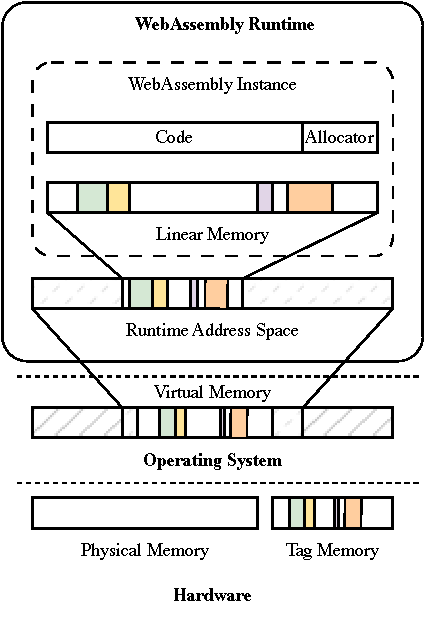
\includegraphics[scale=1]{figures/build/system-design-2}
  \caption{Implementation of the Memory Safety Extension in Wasmtime}
  \label{fig:wasmtime-mte-impl}
\end{figure}

In \cref{fig:wasmtime-mte-impl}, we can see an overview of our implementation of the memory safety extension in wasmtime using \ac{MTE}.
We modified wasmtime and its supporting libraries and extended it with support to parse and process the memory safety extension described in \cref{sec:wasm-extension}.
We added support for \ac{MTE} in the form of new instructions and lowering rules to cranelift, allowing wasmtime to generate \ac{MTE} instructions when compiling for a target that supports them.
We run in \ac{MTE} synchronous mode to catch and stop memory safety violations before their effects become observable to the violating or any other process.

By default, the memory is tagged with one of the tags described in \cref{tab:default-tag}.

\begin{table}
  \centering
  \begin{tabular}{c | c || c}
    \textbf{Memory Safety} & \textbf{MTE Sandboxing} & \textbf{Default Tag} \\
    \hline
    No  & No  & $t \in \{\,0\,\}$ \\
    No  & Yes & $t \in \{\,1, \dots, 15\,\}$ \\
    Yes & No  & $t \in \{\,0\,\}$ \\
    Yes & Yes & $t \in \{\,1\,\}$
  \end{tabular}
  \caption{Default tag $t$ for the linear memory}
  \label{tab:default-tag}
\end{table}

For \ac{MTE}, we store the logical tag directly in the \ac{WASM} index.
However, when assigning the allocation tag, we need to translate the index to an address.
Before assigning tags, we also need to perform explicit bounds checks. Otherwise, we would allow untrusted guest code to set arbitrary tags in the process address space.
In the following paragraphs, we will describe how we lower each of our instructions to an \ac{MTE} backend.

\paragraph{\texttt{segment.new}} To create a new segment, we (1) check that the requested segment is inside the linear memory for the guest, (2) generate a random logical tag and insert it into the index, and (3) set the allocation tag for the segment.
This involves generating a loop that iterates over the size of the segment and setting the tag using \texttt{stzg}, which also zeroes the memory.

\paragraph{\texttt{segment.set\_tag}} To change ownership of a segment, we again (1) check that the requested segment is inside the linear memory for the guest and (2) set the new allocation tag for the segment.
Here, we do not need to create a new, random tag, as we have passed a predefined tag.

\paragraph{\texttt{segment.free}} To invalidate a segment, we (1) check that the requested segment is inside the linear memory for the guest and (2) set the default allocation tag for the segment.
The default tag depends on the configuration and can be taken from \cref{tab:default-tag}.

\paragraph{}
We have implemented several optimizations to ensure our generated code runs efficiently.
When setting the allocation tag for a segment, we generate a loop iterating over the size of the segment.
If the size of the loop is known at compile time, we unroll the loop to tag up to 160\,bytes per iteration to avoid branch instructions.
We chose this tradeoff between code size and reducing the number of branch instructions executed.

When setting an allocation tag, we have three choices:
\begin{enumerate}
  \item \texttt{stg}: Setting the tag for a single tag granule,
  \item \texttt{st2g}: Setting the tag for two tag granules,
  \item \texttt{stzg}: Setting the tag for a single granule and zeroing the granule.
  \item \texttt{stgp}: Setting the tag for a single granule and storing a pair of registers.
\end{enumerate}

To ensure new segments are always zeroed, options 1) and 2) would require an additional memset.
We benchmarked all four variants (see \cref{sec:mte-performance-evaluation}) and chose \texttt{stzg}, as it had the lowest overhead while clobbering one less register compared to \texttt{stgp}.

\subsection{Migration of the Linear Memory}
\label{subsec:migration-of-the-linear-memory}

When resizing the linear memory, the runtime needs to move the existing linear memory to a new region.
If memory safety is enabled, we need to ensure to also migrate the tags from the old region to the new region.
Since each memory granule may be tagged with a distinct tag, we have the choice between two approaches.

\begin{description}
\item[Temporarily disable MTE]
We can disable \ac{MTE} for the whole process, copy the contents and tags of the old linear memory to the new linear memory, and then re-enable \ac{MTE}.

\item[Load the tag for each granule]
We can first load the tag for a granule of memory and then use that tag to perform the memory access to load and then store the 16\,bytes of memory from the old to the new linear memory.
\end{description}

\noindent
We have measured the performance of both approaches in \cref{subsec:migrating-tagged-memory}.

\subsection{\ac{MTE} Sandboxing}
\label{subsec:bounds-checks}

In \cref{fig:system-design-sandboxing}, we showcase an approach that utilizes memory tagging to replace software-based bounds checks.
On module instantiation, the runtime assigns a tag to each instance.
This tag is stored in the heap base address.
Memory access translation then involves adding this tagged heap base address to the accessed index.
Memory belonging to the runtime is always tagged with the zero tag.

However, we face a limitation in the number of sandboxes for this approach.
Since \ac{MTE} only offers up to 16 distinct tags, we are limited to up to 15 different sandboxes within one process, as we need to reserve one tag for the runtime.

\begin{figure}[t]
  \centering
  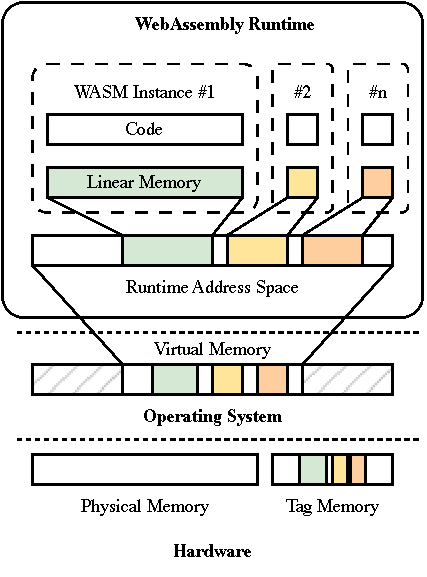
\includegraphics[scale=1]{figures/build/system-design-1}
  \caption{Bounds checks using MTE}
  \label{fig:system-design-sandboxing}
\end{figure}

We can combine this approach with the memory safety extension by further restricting the number of sandboxes in one process and thus freeing up tag bits for the memory safety extension.
For our prototype, we decided to allow just a single instance when combining \ac{MTE} bounds checks and the memory safety extension.
We designate the lowest tag bit to determine whether memory belongs to the runtime or the linear memory.
Since we reserved the zero tag for the runtime, we tag the linear memory with the tag 1.
The remaining three tag bits are used for the memory safety features and can be generated by \texttt{segment.new}.
Thus, memory indices always have an even tag, while the actual memory locations have an odd tag.

There are two challenges we need to take care of:
\begin{enumerate}
  \item Adding a tagged user pointer to the heap base address should be performant and result in the correct tag for the respective memory.
  \item It is crucial to prevent users from creating tags that enable access beyond their allocated memory sandbox.
\end{enumerate}
However, we need to ensure that adding an untrusted index to the heap base does not overflow and thus change the tag, allowing code to escape the sandbox.
Thus, we need to mask the index before the address computation.

Memory accesses are translated by adding the tagged heap base to the tagged index, as shown in \cref{fig:system-design-mem-safety-bounds}.
However, since the memory index is untrusted, an attacker may craft a value that overflows the tag bits when adding it to the heap base, resulting in a tag that allows memory accesses outside the sandbox.
To prevent this, we need to mask the tag bits allocated for the runtime.
\Cref{fig:mte-bounds-checks} shows the masked bits when just \ac{MTE} bounds checking is enabled.
In this case, we allocate all bits for the runtime and mask out the tag bits in the index.
In \cref{fig:mte-bounds-checks-mem-safety}, we see what happens when both \ac{MTE} bounds checking and memory safety are enabled.
Here, we allocate the lowest bit for the runtime while we leave the remaining three for the memory safety extension.
In \cref{tab:tag-mask}, we can see the mask used for each configuration.

\begin{table}
  \centering
  \begin{tabular}{c | c || c}
    \textbf{Memory Safety} & \textbf{MTE Sandboxing} & \textbf{Tag Mask} \\
    \hline
    No  & No  & -- \\
    No  & Yes & \texttt{and 0xF0FF\_FFFF\_FFFF\_FFFF} \\
    Yes & No  & -- \\
    Yes & Yes & \texttt{and 0xFEFF\_FFFF\_FFFF\_FFFF}
  \end{tabular}
  \caption{Tag Mask for the Index.}
  \label{tab:tag-mask}
\end{table}

\begin{figure}[t]
  \centering
  \begin{subfigure}[T]{\textwidth}
    \centering
    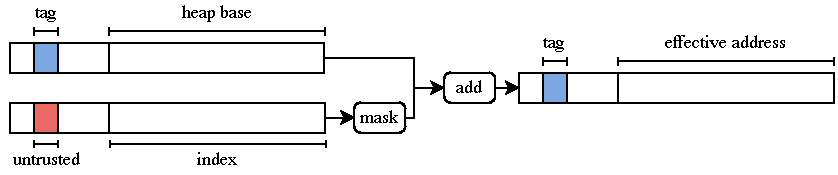
\includegraphics{figures/build/bounds}
    \caption{\ac{MTE} Bounds Checks.}
    \label{fig:mte-bounds-checks}
  \end{subfigure}
  \hfill
  \begin{subfigure}[T]{\textwidth}
    \centering
    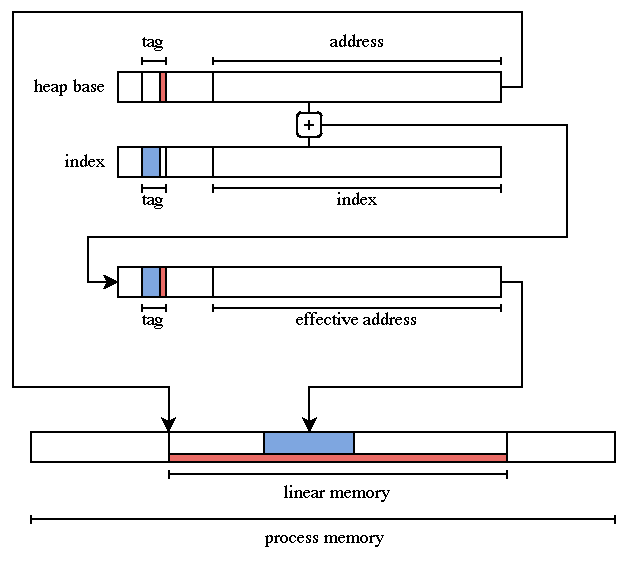
\includegraphics{figures/build/bounds-mem-safety}
    \caption{\ac{MTE} bounds checks with Memory Safety Extension.}
    \label{fig:mte-bounds-checks-mem-safety}
  \end{subfigure}
  \caption{Effective Address Calculation with \ac{MTE} bounds checks.}
  \label{fig:system-design-mem-safety-bounds}
\end{figure}

\paragraph{Excluding Tags from Random Tag Generation}
If we are running with \ac{MTE} bounds checks enabled, we need a way to ensure to exclude certain tags from being generated by instructions such as \texttt{irg} (\textbf{i}nsert \textbf{r}andom ta\textbf{g}) or \texttt{addg} (\textbf{add} ta\textbf{g}).
This can be either specified as an exclude mask via an immediate to the instruction or an include mask via a \texttt{prctl} call, which sets the corresponding register in kernel space.
We chose the latter option and set the include mask at startup time.
In \cref{tab:tag-include-mask}, we list the include masks and included tags for the instructions mentioned above.
If the memory safety extension is disabled, none of these instructions will be emitted, so we do not need to exclude tags from being generated.

\begin{table}
  \centering
  \begin{tabular}{c | c || c | c}
    \textbf{Memory Safety} & \textbf{MTE Sandboxing} & \textbf{Tag Include Mask} & \textbf{Included Tags} \\
    \hline
    No  & No  & -- & -- \\
    No  & Yes & -- & -- \\
    Yes & No  & \texttt{0xffff} & $t \in \{\,1, 2, \dots, 15\,\}$ \\
    Yes & Yes & \texttt{0x5555} & $t \in \{\,2, 4, \dots, 14\,\}$
  \end{tabular}
  \caption{Included Tags for \texttt{irg}, \texttt{addg} instructions depending on configuration.}
  \label{tab:tag-include-mask}
\end{table}

